\chapter{Resilient Distributed Dataset\label{ch:rdd}}

Spark programming model is based on Resilient Distributed Dataset (RDD) abstraction. "An RDD is a read-only,
partitioned collection of records". It is used at application-layer, which enables faster
I/O, since the datasets can be stored in-memory as Java objects. This not only avoids disk writes, but also data
de-serialization. Instead of relying on data replication, RDDs keep lineage information about how they were transformed
from other RDDs.

Measure for encoding entropy is displayed on Equation \ref{eq:entropy}.

\begin{equation}\label{eq:entropy}
  H(X) = \sum_{x\in X}p(x) \log p(x)
\end{equation}

Figure of foobar is displayed on Figure \ref{fig:foobar}.

\begin{figure}[t!]
  \centering
  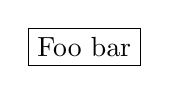
\begin{tikzpicture}
    \node[rectangle,draw] {Foo bar};
  \end{tikzpicture}
  \caption{Lorem ipsum dolot}\label{fig:foobar}
\end{figure}
